\chapter{Preliminarii}

\section{Noțiuni de bază}

Înainte de a ne aprofunda în analiza specifică a acestei lucrări, este important să înțelegem câteva noțiuni fundamentale care stau la baza dezvoltării și implementării unui asistent virtual în domeniul bancar.

\begin{itemize}
    \item \textbf{Chatbot} 

Chatbotul este un program software ce simulează o conversație umană. În mod tradițional, utilizatorii interacționează cu chatbotii prin intermediul unei interfețe textuale, deși unii chatboti moderne pot interacționa și prin comenzi vocale.

Există două tipuri principale de chatboti: chatbotii bazati pe reguli și chatbotii bazati pe învățarea automată. Chatbotii bazati pe reguli sunt proiectați pentru a răspunde la întrebări specifice și sunt programați cu un set de reguli predefinite. Pe de altă parte, chatbotii bazati pe învățare automată se bazează pe algoritmi de inteligență artificială și sunt capabili să învețe din interacțiunile cu utilizatorii.

În industria bancară, chatbotii sunt utilizati în special în serviciul de asistență pentru clienți, unde pot răspunde la întrebări frecvente, pot ajuta la rezolvarea problemelor și pot ghida utilizatorii prin diferite procese.

    \item \textbf{Tehnologia Cloud}

Tehnologia cloud se referă la livrarea de servicii IT prin internet, în loc de a folosi infrastructura fizică locală. Aceasta poate include servicii de calcul, stocare, baze de date, rețelistică, software, analize și inteligență.

Există trei tipuri principale de servicii cloud: Infrastructură ca Serviciu (IaaS), Platformă ca Serviciu (PaaS) și Software ca Serviciu (SaaS). În industria bancară, cloud computing-ul poate ajuta la reducerea costurilor, la îmbunătățirea eficienței operaționale și la scalabilitate.

    \item \textbf{Inteligenta artificială} 

Inteligența Artificială (AI) se referă la simularea inteligenței umane de către mașini, în special sistemele informatice. Sarcinile AI pot include învățarea (abilitatea de a dobândi și aplica cunoștințe și abilități), raționamentul (utilizarea de reguli pentru a ajunge la concluzii aproximative sau definite), auto-corectarea și procesarea limbajului natural.

Chatbotii bazati pe AI, cum ar fi cei dezvoltati cu DialogFlow, pot învăța din interacțiuni și pot îmbunătăți continuu calitatea conversațiilor pe care le au cu utilizatorii.

    \item \textbf{DialogFlow}

DialogFlow, deținut de Google, este o platformă care permite dezvoltatorilor să creeze interfețe de conversație pentru site-uri web, aplicații mobile și platforme populare de mesagerie \cite{sharma2018}. DialogFlow utilizează tehnologia de înțelegere a limbajului natural (NLU - \emph{Natural Language Understanding}) pentru a înțelege și a procesa limbajul uman.

În contextul dezvoltării chatbotilor pentru instituțiile bancare, DialogFlow poate ajuta la crearea de boti care să înțeleagă și să răspundă la cererile utilizatorilor într-un mod mai natural și mai intuitiv.

\end{itemize}

\section{Stadiul actual al subdomeniului}

Implementarea chatbotilor în sistemul bancar reprezintă o inovație semnificativă în modul în care băncile interacționează cu clienții lor. Începând cu Banca Transilvania în 2017, multe alte instituții bancare din România au urmat exemplul și au început să folosească chatboti pentru a îmbunătăți serviciile oferite clienților.

Chatbotii oferă un nivel de disponibilitate non-stop, care este deosebit de valoros într-o industrie precum cea bancară, care necesită suport pentru clienți la orice oră. Prin eliminarea nevoii de interacțiune umană pentru a rezolva probleme comune, chatbotii permit băncilor să economisească resurse și să se concentreze pe probleme mai complexe. Acești asistenți virtuali pot răspunde rapid la întrebări, pot rezolva probleme și pot oferi asistență în tranzacții financiare, îmbunătățind astfel satisfacția generală a clienților.

Cu toate acestea, în ciuda progreselor semnificative în adoptarea tehnologiei chatbot în industria bancară, există încă multe oportunități de explorare și îmbunătățire. Un domeniu cheie de cercetare este îmbunătățirea înțelegerii naturale a limbajului de către chatboti. Deși chatbotii actuali sunt capabili să gestioneze o serie de interacțiuni de bază, abilitatea lor de a înțelege nuanțele și complexitatea limbajului uman este limitată.

Un alt domeniu de potențială îmbunătățire este personalizarea și adaptabilitatea. În prezent, majoritatea chatbotilor bancari folosesc algoritmi pre-programați pentru a răspunde la interacțiunile utilizatorilor. Cu toate acestea, există oportunități semnificative pentru utilizarea tehnologiilor avansate de AI, cum ar fi învățarea profundă, pentru a dezvolta chatboti care pot învăța și se pot adapta la comportamentul și preferințele individuale ale utilizatorilor.

\begin{figure}[h] % h = here, adica pune figura fix unde e textul
    \centering
    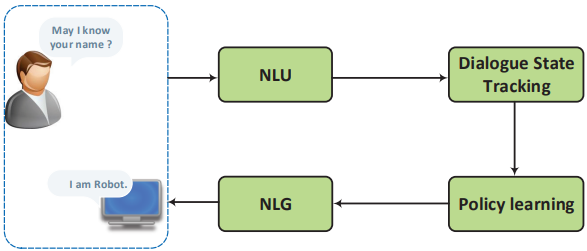
\includegraphics[width=0.8\textwidth]{traditional-pipeline}
    \caption{Pipeline general pentru sisteme orientate pe task-uri \cite{chen_liu_yin_tang_dialogue_2017}}
    \label{fig:traditional-pipeline}
\end{figure}

În plus, există încă multe provocări legate de securitate și confidențialitate care trebuie abordate înainte ca chatbotii să fie adoptați pe scară largă în industria bancară. Acestea includ protejarea datelor personale și financiare ale utilizatorilor și asigurarea că chatbotii nu pot fi utilizați pentru activități frauduloase.

În concluzie, în timp ce adoptarea chatbotilor în sistemul bancar a făcut progrese remarcabile în ultimii ani, există încă multe oportunități de cercetare și dezvoltare în acest domeniu. Pe măsură ce tehnologia continuă să avanseze, este de așteptat ca chatbotii să devină un element tot mai integral al serviciilor bancare.

\section{Obiectivele lucrării în contextul subdomeniului}

Obiectivul principal al acestei lucrări este de a investiga posibilitățile pe care tehnologia chatbot și serviciile cloud le oferă în contextul sistemului bancar. În particular, accentul este pus pe implementarea unui model de chatbot bazat pe platforma DialogFlow, cu suport pentru limbajul de programare C++. C++ este un limbaj de programare popular, cunoscut pentru eficiența și puterea sa, fiind astfel un candidat potrivit pentru dezvoltarea unui chatbot robust și eficient.

În actualul stadiu de dezvoltare a tehnologiei chatbot, această lucrare vizează să contribuie la progresul subdomeniului, prin oferirea unei viziuni detaliate asupra procesului de implementare a unui chatbot în serviciile bancare, lucrarea speră să aducă o valoare semnificativă domeniului.

În plus, lucrarea explorează și potențialele căi de îmbunătățire și adaptare a chatbotilor. O astfel de direcție ar putea fi folosirea de tehnologii avansate de AI, cum ar fi învățarea profundă, pentru a dezvolta chatboti care pot învăța și se pot adapta la comportamentul și preferințele individuale ale utilizatorilor. Prin urmare, acest studiu își propune să deschidă calea către o utilizare mai extinsă și mai eficientă a tehnologiei chatbot în industria bancară.

Pe de altă parte, această lucrare se concentrează și asupra cloud computing-ului, o tehnologie care a revoluționat modul în care datele și serviciile sunt gestionate. Cu ajutorul cloud computing-ului, chatbotii pot fi ușor scalabili, ceea ce înseamnă că pot servi un număr mare de utilizatori simultan, fără a compromite performanța. În plus, cloud computing-ul facilitează actualizările și îmbunătățirile continuu, fără întreruperi majore ale serviciului \cite{mell_grance2011}.

În concluzie, această lucrare are ca scop principal să demonstreze cum tehnologiile moderne, precum chatbotii și cloud computing-ul, pot transforma modul în care băncile interacționează cu clienții lor. Se urmărește evidențierea beneficiilor potențiale ale utilizării agenților conversaționali pentru optimizarea proceselor și serviciilor bancare, în speranța de a stimula o adoptare mai largă a acestor tehnologii în industria bancară.